Για να διασχίσει ένα αυτόνομο επίγειο ρομπότ το περιβάλλον του πρέπει να είναι
διαθέσιμες μία σειρά από προϋποθέσεις και λειτουργίες. Πρώτον είναι αναγκαία η
ύπαρξη ενός στόχου για να φτάσει το ρομπότ. Αυτός ο στόχος είναι συνήθως η
επιθυμητή τελική στάση του στον $2D$ χώρο ($[x, y, \theta]$---σχήμα
\ref{fig:pose_figure}). Στη συνέχεια πρέπει να χρησιμοποιηθεί ένας αλγόριθμος
ικανός να λάβει ως είσοδο τη ρομποτική αντίληψη για τον περιβάλλοντα κόσμο
(συνήθως ένας $2D$ ή $3D$ χάρτης), καθώς και την εκτίμηση για την αρχική στάση
του ρομπότ, ώστε να είναι δυνατή η εκτίμηση της στάσης του ρομπότ ενόσω αυτό
κινείται αυτόνομα προς τον ανωτέρω στόχο (pose tracking---ενότητα
\ref{subsec:01_01_02_2}).  Έπειτα απαιτείται η ύπαρξη ενός γεωμετρικού
μονοπατιού το οποίο, εάν ακολουθηθεί από το ρομπότ, θα το οδηγήσει από την
αρχική στην επιθυμητή του στάση. Αυτό το μονοπάτι παράγεται από έναν αλγόριθμο
χάραξης μονοπατιών, του οποίου το αντικείμενο είναι το σύνολο του (στατικού)
χάρτη. Τέλος, ένας ελεγκτής κίνησης είναι απαραίτητος, ο οποίος θεωρεί ως
εισόδους του το μονοπάτι, την τρέχουσα στάση του ρομπότ, και την τοπική του
αντίληψη,\footnote{Με τον όρο τοπική αντίληψη εννοούνται τα ακατέργαστα
αισθητηριακά δεδομένα που αντιπροσωπεύουν τις δυναμικές μεταβολές του
περιβάλλοντος, σε αντιδιαστολή με τον στατικό συνολικό χάρτη.} και παράγει
ταχύτητες κινητήρων έτσι ώστε να οδηγηθεί το ρομπότ στο να ακολουθήσει το
μονοπάτι. Ταυτόχρονα, είναι αρμοδιότητα τού τελευταίου να πλοηγείται το ρομπότ
με την μεγαλύτερη δυνατή ασφάλεια (υποθέτοντας ότι το ρομπότ θα πρέπει να
αποφεύγει συγκρούσεις με στατικά ή κινούμενα αντικείμενα, αν και αυτό δεν
αποτελεί πάντοτε προϋπόθεση \cite{Gandhi2017}).

Σε αυτή την ενότητα παρέχεται μία επισκόπηση των αλγορίθμων χάραξης μονοπατιών
της βιβλιογραφίας, των ελεγκτών κίνησης για επίγειες κινητές βάσεις, καθώς και
των υλοποιήσεών τους σε υπολογιστή με το λειτουργικό σύστημα \texttt{ROS}.

%%%%%%%%%%%%%%%%%%%%%%%%%%%%%%%%%%%%%%%%%%%%%%%%%%%%%%%%%%%%%%%%%%%%%%%%%%%%%%%%
\subsection{Αλγόριθμοι χάραξης μονοπατιών}
\label{subsection:02_01_02:01}

Όσον αφορά στους αλγορίθμους χάραξης μονοπατιών αυτοί συνήθως ανήκουν σε μία
από τις παρακάτω έξι κύριες αλγοριθμικές οικογένειες: \textit{Γράφοι
Ορατότητας} (Visibility Graphs), \textit{Τεχνικές Βασισμένες στη
Σκελετοποίηση}, \textit{Πιθανοτικoί Οδικοί Χάρτες} (Probabilistic
Roadmaps---PRM), \textit{Τυχαία Δένδρα Ταχείας Εξερεύνησης} (Rapidly exploring
Random Trees---RRT), \textit{Πλέγματα Κατάστασης} (State Lattices), και
\textit{Συναρτήσεις Πλοήγησης} (Navigation Functions---NF).

Οι Γράφοι Ορατότητας ήταν μία από τις πρώτες μεθόδους σχεδιασμού μονοπατιών.
Προτάθηκαν από τους Losano-Perez και Wesley το 1979 \cite{Lozano-Perez1979},
και περιγράφουν μια μέθοδο δημιουργίας μονοπατιών σε κυρτά περιβάλλοντα, όπου
τα εμπόδια μετασχηματίζονται με τρόπο τέτοιο ώστε να απεικονίζουν περιοχές που
δεν μπορούν να διασχιστούν λόγω των γεωμετρικών περιορισμών του αποτυπώματος
του ρομπότ. Μετά την κατασκευή του γράφου ορατότητας, ο οποίος περιέχει ως
κόμβους τα μετασχηματισμένα εμπόδια, εφαρμόζεται ένας αλγόριθμος αναζήτησης για
τη δημιουργία της τελικής διαδρομής. Όπως περιγράφεται στα \cite{Ghosh2007} και
\cite{Ghosh2013} οι γράφοι ορατότητας υποφέρουν από υψηλές απαιτήσεις σε
υπολογιστικούς πόρους και από την πολυπλοκότητα των γεωμετρικών περιορισμών των
εμποδίων. Ως εκ τούτων, έχουν προταθεί άλλες προσεγγίσεις για την αντιμετώπιση
αυτών των ζητημάτων \cite{Kim2011}.

Μεταξύ των τεχνικών σκελετοποίησης το Γενικευμένο Διάγραμμα Voronoi
(Generalised Voronoi Diagram---GVD) είναι ο κυρίαρχος αλγόριθμος που
χρησιμοποιείται προκειμένου να παραχθεί ένας σκελετός του ελεύθερου χώρου στον
οποίο κινείται το ρομπότ, και συνεπώς μονοπατιών πλοήγησης των οποίων τα σημεία
ισαπέχουν από τα εμπόδια του περιβάλλοντος. Παραδείγματα χρήσης του GVD σε
αλγορίθμους χάραξης μονοπατιών αναφέρονται (α) στο \cite{Garrido2006}, όπου το
GVD ακολουθείται από την εφαρμογή της μεθόδου Fast Marching για την
ελαχιστοποίηση του μήκους της διαδρομής, (β) στο \cite{Bhattacharya2007}, όπου
το GVD χρησιμοποιείται για τη δημιουργία μιας ομαλής διαδρομής που εάν
ακολουθηθεί κατά γράμμα δεν επιφέρει συγκρούσεις του ρομπότ με το περιβάλλον
του, και (γ) στο \cite{Ok2013}, το οποίο εισάγει τα Πεδία Αβεβαιότητας Voronoi
(VUF), και που συνδυάζει το GVD για την κατασκευή μονοπατιών και έναν ελεγκτή
κίνησης για την πλοήγηση του οχήματος.

Μια από τις πιο διάσημες οικογένειες αλγορίθμων σχεδιασμού διαδρομής είναι αυτή
των Πιθανοτικών Οδικών Χαρτών. Η ιδέα τους είναι απλή: πραγματοποιείται
δειγματοληψία στον ελεύθερο χώρο του χάρτη του περιβάλλοντος και δημιουργείται
ένας γράφος του οποίου οι ακμές είναι ασφαλείς για προσπέλαση. Στη συνέχεια
εφαρμόζεται ένας αλγόριθμος αναζήτησης στον γράφο για την εύρεση της διαδρομής
που εμφανίζει ελάχιστο κόστος με βάση τη μετρική του μήκους του συνολικού
μονοπατιού από την αρχική προς την τελική στάση. Τα PRM εισήχθησαν αρχικά από
τους Kavraki κ.α. \cite{Kavraki1996}, ωστόσο έχουν προταθεί διάφορες
τροποποιήσεις, όπως (α) στο \cite{Nissoux}, όπου οι έννοιες των Γράφων
Ορατότητας χρησιμοποιούνται για την ενίσχυση του PRM, (β) στο \cite{Bohlin2000}
που εισάγει τον αλγόριθμο Lazy PRM, ο οποίος ελαχιστοποιεί δυναμικά τις
συνδέσεις του γράφου, και (γ) στο \cite{Hsua} όπου προτείνεται ο υβριδικός PRM,
δηλαδή ένας συνδυασμός διαφορετικών PRM ανάλογα με τις ιδιότητες του
περιβάλλοντος.

Μια άλλη μεθοδολογία σχεδιασμού μονοπατιών είναι αυτή των Τυχαίων Δένδρων
Ταχείας Εξερεύνησης, που προτάθηκε αρχικά από τον La Valle το 1998
\cite{Lavalle1998}. Τα RRT δημιουργούν επαναληπτικά δενδροειδείς δομές,
ξεκινώντας από έναν κόμβο-ρίζα και τερματίζουν όταν ένα φύλλο φτάσει στον
επιθυμητό στόχο. Υπάρχουν διάφορες τροποποιήσεις του, όπως, μεταξύ άλλων, το
Execution Extended RRT (ERRT) \cite{Bruce}, τα αμφίδρομα RRT \cite{Martin2007},
Cell-RRT \cite{Guitton2009}, RRT* \cite{Karaman2010}, και T-RRT
\cite{Jaillet2010}.

Ο σχεδιασμός μονοπατιών σε Πλέγματα Καταστάσεων εμφανίστηκε το 2005 από τους
Pivtoraiko και Kelly \cite{MikhailPivtoraiko2005}. Ένα πλέγμα καταστάσεων είναι
ένας χώρος αναζήτησης που περιλαμβάνει ένα διακριτοποιημένο σύνολο από τις
προσβάσιμες-εφικτές καταστάσεις ενός συστήματος (του κινηματικού μοντέλου του
ρομπότ εν προκειμένω), το οποίο μπορεί να κωδικοποιήσει ακολουθήσιμα-εφικτά
μονοπάτια. Τα μονοπάτια σχηματίζονται από τοπικές συνδέσεις μεταξύ καταστάσεων
που συμμορφώνονται στους εκάστοτε κινηματικούς περιορισμούς της κινητής βάσης,
και στους περιορισμούς που θέτει ο περιβάλλον χώρος. Μετά την ανάπτυξη του χώρου
αναζήτησης δημιουργείται ένα σύνολο χωρικά διακριτών μονοπατιών. Αυτός ο χώρος
κωδικοποιεί τις τοπικές συνδέσεις και εξαλείφει τους πλεονασμούς έτσι ώστε ένα
ερώτημα σχεδιασμού στο συνδεδεμένο γράφημα αναζήτησης να μπορεί να εκτελεστεί
με αποδοτικό τρόπο.

Οι Συναρτήσεις Πλοήγησης είναι μια ειδική κατηγορία Συναρτήσεων Δυναμικού για
την πλοήγηση ρομπότ κινητής βάσης \cite{Latombe1991}. Η συναρτήσεις δυναμικού
προϋποθέτουν έναν γνωστό χάρτη, και αποδίδουν μια τιμή δυναμικού σε κάθε σημείο
του (σε χάρτες που βασίζονται σε ορόσημα) ή σε κάθε κελί πλέγματος (σε χάρτες
που βασίζονται σε πλέγμα): κάθε ένα από αυτά λαμβάνει τιμή δυναμικού αντιστρόφως
ανάλογη με την απόστασή του από ένα εμπόδιο. Αντίθετα, στη στάση του στόχου
αποδίδεται χαμηλή τιμή δυναμικού. Η αρχή του δυναμικού πεδίου είναι ελκυστική
λόγω της απλότητας και της κομψότητάς της, ωστόσο, στη βιβλιογραφία αναφέρεται
ένας αριθμός ουσιαστικών ελλείψεων \cite{Koren}\cite{Ge2000}, όπως η
ευαισθησία της μεθόδου στο να παγιδεύει το ρομπότ σε τοπικά ελάχιστα, και η
αύξηση των ταλαντώσεων όταν ένα ρομπότ πλησιάζει εμπόδια ή στενά περάσματα. Οι
Συναρτήσεις Πλοήγησης προσπαθούν να ξεπεράσουν αυτά τα προβλήματα: είναι
συναρτήσεις (α) για τις οποίες το δυναμικό του στόχου λαμβάνει μηδενική τιμή ή,
εάν ο στόχος είναι απρόσιτος, άπειρη τιμή, και (β) που έχουν μονοτονική κλίση,
δηλαδή δεν περιλαμβάνουν τοπικά ελάχιστα, εκτός από αυτό του στόχου. Ωστόσο, η
μέθοδος της συνάρτησης πλοήγησης μπορεί παρουσιάσει αργή σύγκλιση, ιδίως όταν
το περιβάλλον του ρομπότ περιλαμβάνει στενά περάσματα, και επομένως απαιτεί
προσαρμοσμένη ρύθμιση \cite{Kowalczyk2019}. Επιπλέον, στην χώρους υψηλών
διαστάσεων, όπου τα σχήματα του ρομπότ ή των εμποδίων είναι πολύπλοκα, το
υπολογιστικό κόστος αυξάνεται απότομα \cite{Park2016}.

%%%%%%%%%%%%%%%%%%%%%%%%%%%%%%%%%%%%%%%%%%%%%%%%%%%%%%%%%%%%%%%%%%%%%%%%%%%%%%%%
\subsection{Ελεγκτές κίνησης}
\label{subsection:02_01_02:02}

Αφού δημιουργηθεί το μονοπάτι που συνδέει την αρχική με την επιθυμητή στάση του
ρομπότ, ένας ελεγκτής κίνησης πρέπει να χρησιμοποιηθεί προκειμένου το ρομπότ να
ακολουθήσει το μονοπάτι στον πραγματικό χώρο, με βάση μετρήσεις από τους
εξωδεκτικούς του αισθητήρες. Ο ελεγκτής πρέπει ταυτόχρονα να βεβαιωθεί ότι
αποφεύγει τόσο τα στατικά όσο και τα δυναμικά εμπόδια του περιβάλλοντος του
ρομπότ Οι ελεγκτές κίνησης ανήκουν κατά κύριο λόγο σε μία από πέντε οικογένειες
προσεγγίσεων: \textit{Ιστογράμματα Διανυσματικών Πεδίων} (Vector-Field
Histograms--VFH), \textit{Προσέγγιση Δυναμικού Παραθύρου} (Dynamic Window
Approach---DWA), \textit{Δένδρα Πλοήγησης Κενών} (Gap Navigation Trees---GNT),
\textit{Προσέγγιση Πλοήγησης με Διαγράμματα Εγγύτητας} (Nearness Diagram
navigation approach---ND), και \textit{Ελαστικής Ζώνης} (Elastic Band).

Ένας από τους παλαιότερους ελεγκτές κίνησης είναι τα Ιστογράμματα Διανυσματικού
Πεδίου, που προτάθηκαν το 1991 από τους Borenstein και Koren
\cite{Borenstein1991}. Τα VFH δημιουργούν ένα πολικό ιστόγραμμα σε σχέση με τον
προσανατολισμό του ρομπότ μέσω των μετρήσεων των αισθητήρων του, αποδίδοντας σε
κάθε προσανατολισμό την πιθανότητα η κατεύθυνση αυτή να είναι κατειλημμένη από
εμπόδιο. Στη συνέχεια εντοπίζονται επαρκώς μεγάλα ανοίγματα για να μπορεί το
ρομπότ να πλοηγηθεί με ασφάλεια μέσα από αυτά, και υπολογίζεται μια συνάρτηση
κόστους για κάθε άνοιγμα, όπου και τελικά επιλέγεται αυτό με το μικρότερο
κόστος.  Βελτιώσεις των VFH είναι τα VFH+, τα οποία ενσωματώνουν τοξοειδείς
τοπικές τροχιές, σε αντίθεση με τις ευθείες γραμμές των VFH \cite{Ulrich}, και
τα VFH* τα οποία επαληθεύουν ότι μια υποψήφια κατεύθυνση οδηγεί το ρομπότ
\textit{γύρω} από ένα εμπόδιο, χρησιμοποιώντας τον αλγόριθμο A* και τις
κατάλληλες συναρτήσεις κόστους και ευρηστικών συναρτήσεων \cite{Ulricha}.

Μια άλλη διάσημη προσέγγιση είναι η Προσέγγιση Δυναμικού Παραθύρου, που
προτάθηκε από τους Fox, Burgard, και Thrun \cite{Fox1997}. Η DWA δειγματοληπτεί
το τοπικό περιβάλλον του ρομπότ με πιθανές τροχιές που προκύπτουν άμεσα από το
κινηματικό μοντέλο του, υπολογίζοντας ένα κόστος για κάθε δείγμα. Η συνάρτηση
αυτή περιλαμβάνει την κατεύθυνση του ρομπότ σε σχέση με τον επιθυμητό στόχο,
την απόσταση της τροχιάς του από το πλησιέστερο εμπόδιο, και την προηγούμενη
γραμμική ταχύτητα προκειμένου να ληφθεί υπόψη η αδράνεια του σώματος του. Στη
συνέχεια το σύνολο ταχυτήτων που μεγιστοποιεί μια αντικειμενική συνάρτηση
επιλέγεται για εφαρμογή στους κινητήρες του.

Τα Δένδρα Πλοήγησης Κενών είναι δενδροειδείς δομές που δημιουργούνται από
τρέχουσες μετρήσεις των αισθητήρων του ρομπότ που κωδικοποιούν διαδρομές από
την τρέχουσα θέση του ρομπότ σε οποιοδήποτε σημείο του περιβάλλοντος
\cite{Tovar2005}. Ένα GNT ενημερώνεται καθώς το ρομπότ κινείται, και παράγει
βέλτιστες διαδρομές εάν το περιβάλλον είναι απλά συνδεδεμένο, υπό την
προϋπόθεση ότι τα όρια του περιβάλλοντος είναι ομαλά, αφού προσπαθεί να
εντοπίσει ``κενά" στις μετρήσεις των αισθητήρων.

Μία άλλη προσέγγιση ελεγκτών κίνησης ξεκίνησε το 2004 με την Προσέγγιση
Πλοήγησης με Διάγραμμα Εγγύτητας από τους Minguez και Montano \cite{Mingueza}.
Η μεθοδολογία ND παράγει αρχικά δύο διαγράμματα εγγύτητας: το PND (από το
κεντρικό σημείο του ρομπότ) και το RND (από τα άκρα του ρομπότ) για την
αναπαράσταση των πληροφοριών σχετικά με την εγγύτητα των εμποδίων σε αυτό. Τόσο
το PND όσο και το RND αναλύονται περαιτέρω, και ειδικά τμήματα και κενά
ασφαλείας υπολογίζονται, με βάση τα οποία το ρομπότ λαμβάνει μια κατάσταση
ασφαλείας μεταξύ πέντε διαθέσιμων. Τελικά αξιολογούνται πέντε νόμοι κίνησης,
σύμφωνα με την κατηγορία ασφαλείας του ρομπότ, με αποτέλεσμα τις κατάλληλες
εντολές ταχύτητας τη δεδομένη χρονική στιγμή. Η μεθοδολογία ND+ προτείνει την
προσθήκη ενός έκτου σεναρίου για την εξισορρόπηση της διαίρεσης των νόμων
κίνησης, αυξάνοντας την ομαλότητα των μεταβάσεων μεταξύ ορισμένων από τα
σενάρια \cite{Minguez2004a}. Τέλος, η πλοήγηση SND (Smooth Nearness-Diagram)
είναι μια εξέλιξη της ND+, όπου ένας μόνο νόμος κίνησης εφαρμόζεται σε όλες τις
πιθανές καταστάσεις του ρομπότ γύρω από τα εμπόδια, αφαιρώντας την εμφάνιση
απότομων μεταβατικών φαινομένων όταν το ρομπότ πλοηγείται κοντά σε εμπόδια
\cite{Durham2008}.

Η προσέγγιση Ελαστικής Ζώνης των Quinlan και Khatib \cite{Quinlan} γεφυρώνει το
μονοπάτι προς ακολούθηση με τη θεωρία ελέγχου: με βάση ένα συνολικό μονοπάτι ο
ελεγκτής κίνησης παράγει μια παραμορφώσιμη διαδρομή σε πραγματικό χρόνο, έτσι
ώστε οι αλλαγές στο περιβάλλον (που ανιχνεύονται από τους αισθητήρες του
ρομπότ), οι αβεβαιότητες στις μετρήσεις, το μοντέλο αβεβαιότητας του
κινηματικού μοντέλου, και τα κινούμενα αντικείμενα να ενσωματώνονται στον
σχεδιασμό και την ακολούθηση της προγραμματισμένης διαδρομής. Για την επίτευξη
των στόχων του (ένας από τους οποίους είναι η διατήρηση της ακεραιότητας της
προγραμματισμένης διαδρομής), η προσέγγιση βασίζεται σε τεχνητές δυνάμεις:
προκαθορισμένες εσωτερικές δυνάμεις συστέλλουν τη διαδρομή και την καθιστούν
πιο ομαλή, ενώ εξωτερικές δυνάμεις διατηρούν τον διαχωρισμό από τα εμπόδια.
Ωστόσο, η αρχική προσέγγιση δεν ενσωματώνει ρητά χρονικούς περιορισμούς ή
περιορισμούς που επιτάσσονται από το ίδιο το κινηματικό μοντέλο του ρομπότ. Μια
επέκταση της αρχικής προσέγγισης, που παραμορφώνει τις τροχιές αλλά όχι τα
προγραμματισμένα μονοπάτια, παρουσιάζεται στο \cite{Kurniawati2007}.

Η προσέγγιση Χρονισμένης Ελαστικής Ζώνης (Timed-Elastic Band)
\cite{ChristophRoesmann}, από την άλλη πλευρά, εμπνευσμένη από την ιδέα της
μεθόδου της Ελαστικής Ζώνης, λαμβάνει υπόψη τόσο τους χρονικούς περιορισμούς
όσο και τους περιορισμούς του κινηματικού μοντέλου της κινητής βάσης. Η αρχική
προσέγγιση παρέχει σε πραγματικό χρόνο τον προγραμματισμό της τροχιάς για
ρομπότ με διαφορική κίνηση. Μιμούμενη έναν ελεγκτή πρόβλεψης μέσω μοντέλου
(Model Predictive Controller), αναδιαμορφώνει το σχεδιασμό της τροχιάς και τον
υπολογισμό ταχυτήτων σε ένα πρόβλημα βελτιστοποίησης που υπόκειται σε
κινηματοδυναμικούς περιορισμούς και περιορισμούς αποφυγής εμποδίων, ενώ
ταυτόχρονα λαμβάνει υπόψη και το συνολικό χρόνο πλοήγησης. Μια επέκταση της
προσέγγισης Χρονισμένης Ελαστικής Ζώνης παρουσιάζεται στο \cite{Rosmann2017},
όπου παρουσιάζεται μια πιο γενική διατύπωση, επεκτείνοντάς την στην υποστήριξη
κινηματικών μοντέλων τύπου Ackermann.


%%%%%%%%%%%%%%%%%%%%%%%%%%%%%%%%%%%%%%%%%%%%%%%%%%%%%%%%%%%%%%%%%%%%%%%%%%%%%%%%
\subsection{Αυτόνομη πλοήγηση με το \texttt{ROS}}
\label{subsection:02_01_02:03}

\begin{figure}\centering
  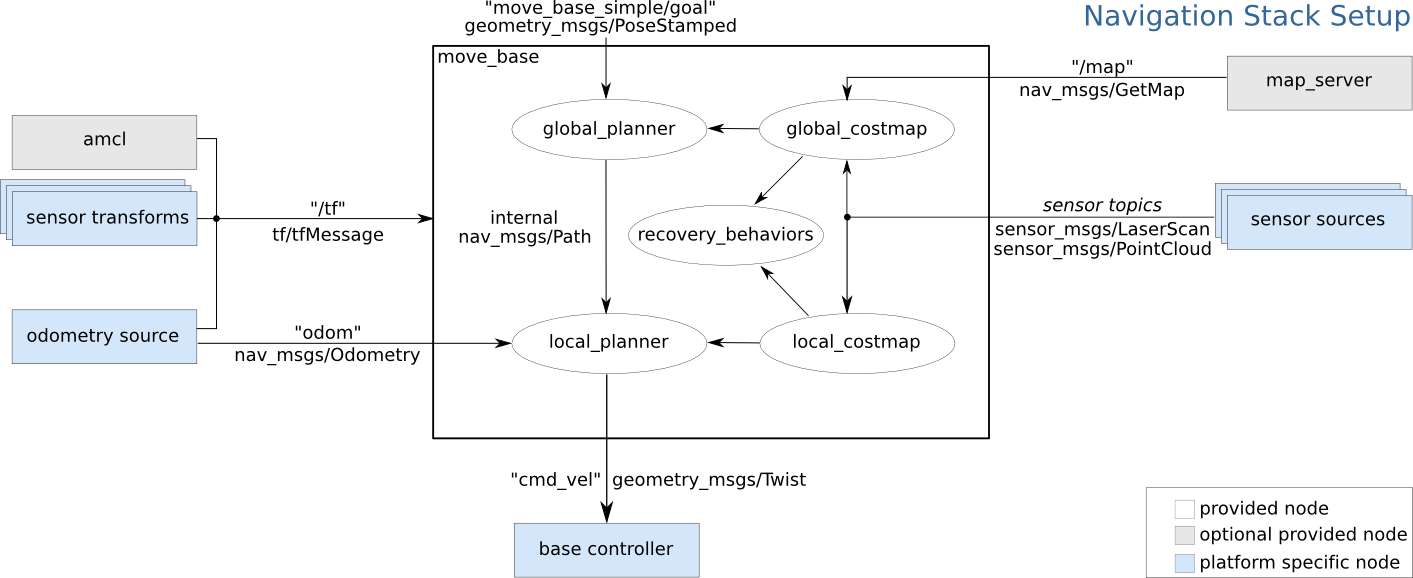
\includegraphics[width=\textwidth]{./figures/parts/01/chapters/03/sections/01/move_base.png}
  \caption{\small Εποπτική άποψη του λογισμικού αυτόνομης πλοήγησης
           \texttt{move\_base}. Πηγή: \url{http://wiki.ros.org/move\_base}}
  \label{fig:movebase}
\end{figure}

Το \texttt{ROS} έχει γίνει ευρέως δημοφιλές στην κοινότητα της ρομποτικής καθώς
προσφέρει μια πληθώρα δωρεάν πακέτων, από ερευνητικές ομάδες όλου του κόσμου.
Προσφέρει δυνατότητες πλοήγησης με τη μορφή \textit{στοιβών} (stacks), δηλαδή
συλλογών πακέτων λογισμικού. Το πιο γνωστό και συχνά χρησιμοποιούμενο από αυτά
είναι το \texttt{\textbf{move\_base}}, το οποίο εσωτερικά χρησιμοποιεί έναν
αλγόριθμο χάραξης μονοπατιών και έναν ελεγκτή κίνησης για να φέρει εις πέρας
το έργο της αυτόνομους πλοήγησης ρομπότ κινητής βάσης. Στην εσωτερική
ονοματολογία του \texttt{ROS} αυτά τα δύο συστατικά ονομάζονται αντίστοιχα
\textit{global planner} και \textit{local planner}. Το \texttt{move\_base}
παίρνει πληροφορίες από την οδομετρία, μετρήσεις από αισθητήρες, και μια
στάση-στόχο, και εξάγει ασφαλείς εντολές ταχύτητας προς είσοδο στους κινητήρες
κινητής βάσης.\footnote{\url{http://wiki.ros.org/navigation}}

Ένα υψηλού επιπέδου διάγραμμα αρχιτεκτονικής της στοίβας πλοήγησης
απεικονίζεται στο σχήμα \ref{fig:movebase}. Κοιτώντας το \texttt{move\_base} ως
ένα μαύρο κουτί, αυτό εξάγει ταχύτητες κινητήρων, και προϋποθέτει την ύπαρξη
των ακόλουθων εισόδων, είτε σε μορφή μηνυμάτων \texttt{ROS} (δομημένα δεδομένα)
ή μετασχηματισμών (σχέσεις μεταξύ συστημάτων αναφοράς):

\begin{itemize}
  \item Την εκτιμώμενη στάση του ρομπότ με τη μορφή ενός μετασχηματισμού μεταξύ
        του οδομετρικού συστήματος αναφοράς του ρομπότ και του συστήματος
        αναφοράς του χάρτη, που παρέχεται εδώ από το πακέτο
        \texttt{amcl}\footnote{\url{http://wiki.ros.org/amcl}}.
        AMCL σημαίνει Adaptive Monte Carlo Localisation
        \cite{Fox2001,Grisetti2007} και είναι επί του παρόντος ο de facto
        αλγόριθμος παρακολούθησης της στάσης ενός ρομπότ μέσα στον δισδιάστατο
        χώρο στο \texttt{ROS}
  \item Πληροφορίες οδομετρίας και (προαιρετικά) τον χάρτη του περιβάλλοντος
  \item Δεδομένα απόστασης είτε από έναν αισθητήρα αποστάσεων τύπου lidar, είτε
        από έναν αισθητήρα που μπορεί να εξάγει νέφη σημείων σε τρεις
        διαστάσεις, όπως μια κάμερα βάθους
  \item Τους μετασχηματισμούς μεταξύ των συστημάτων αναφοράς
        των αισθητήρων και των τελικών στοιχείων (effectors) του ρομπότ
        χρησιμοποιώντας τον μηχανισμό μετασχηματισμού του \texttt{ROS}
        (\texttt{tf})
\end{itemize}

Επιπλέον, το \texttt{ROS} προσφέρει την αναπαράσταση του περιβάλλοντος με τη
μορφή χαρτών κόστους (costmaps), που περιλαμβάνουν πληροφορίες σχετικά με τη
δυνατότητα διέλευσης του ρομπότ μέσα στο περιβάλλον του και μέσα στον χάρτη
αυτού, με βάση το αποτύπωμα του ρομπότ και τα στατικά και δυναμικά εμπόδια
(υποθέτοντας ότι είναι πιο δαπανηρό να να κινηθεί κοντά σε εμπόδια). Όταν
θεωρείται ως λευκό κουτί, το \texttt{move\_base} περιλαμβάνει:

\begin{itemize}
  \item Έναν ολικό χάρτη κόστους (global costmap), που αναπαριστά το κόστος
        διέλευσης πλησίον των στατικών εμποδίων του χάρτη
  \item Έναν τοπικό χάρτη κόστους (local costmap), ο οποίος δημιουργείται και
        ανανεώνεται σε πραγματικό χρόνο στην άμεση γειτονιά του ρομπότ, και που
        βασίζεται στις μετρήσεις των εξωδεκτικών αισθητήρων, προκειμένου να
        αντιμετωπίσει τα στατικά και δυναμικά εμπόδια του πραγματικού
        περιβάλλοντός του
  \item Έναν αλγόριθμο χάραξης μονοπατιών (global planner), ο οποίος λαμβάνει
        ως είσοδο μία στάση-στόχο, και τον ολικό χάρτη κόστους, και παράγει το
        γεωμετρικό μονοπάτι που ενώνει την αρχική στάση του ρομπότ με την
        επιθυμητή
  \item Έναν ελεγκτή κίνησης (local planner), ο οποίος δέχεται ως είσοδο το ως
        άνω μονοπάτι και τον τοπικό χάρτη κόστους, και υπολογίζει εντολές
        ταχύτητας
  \item Μια ενότητα που ονομάζεται συμπεριφορές ανάκτησης (recovery\_behaviours)
        που δέχεται και τους δύο χάρτες κόστους ως είσοδο, εντοπίζει πότε το
        ρομπότ δεν μπορεί να προχωρήσει με την επιθυμητή ταχύτητα, και
        εφαρμόζει προκαθορισμένα σύνολα κινήσεων, με στόχο την ``απεγκλωβισμό"
        του. Αυτές οι ενέργειες ενεργοποιούνται κάθε φορά που (α) το ρομπότ
        γίνεται αντιληπτό ότι ταλαντώνεται, (β) ένα σχέδιο κίνησης δεν έχει
        ληφθεί για πάνω από κάποιο χρονικό διάστημα, ή (γ) ο ελεγκτής κίνησης
        έχει αποτύχει να εξάγει έγκυρες εντολές ταχύτητας για ένα καθορισμένο
        χρονικό διάστημα. Συγκεκριμένα, το \texttt{move\_base} εφαρμόζει δύο
        είδη ανάκτησης του ελέγχου του ρομπότ: (α) μια περιστροφή $360$ μοιρών
        που στοχεύει στην εκκαθάριση του τοπικού χάρτη κόστους από τυχόν
        ψευδείς μετρήσεις (ψευδώς θετικά αντιληπτά εμπόδια) και (β) μια
        επαναφορά του χάρτη κόστους που καθαρίζει την στοίβα πλοήγησης,
        επαναφέροντάς τον στον στατικό χάρτη έξω από τα όρια μιας δεδομένης
        ακτίνας μακριά από το
        ρομπότ\footnote{\url{http://wiki.ros.org/clear\_costmap\_recovery}}. Η
        τελευταία χρησιμοποιείται συνήθως πολλαπλές φορές και σε έναν ιεραρχικό
        τρόπο, ξεκινώντας από κάποια ακτίνα εντός του ημιπλάτους του τοπικού
        χάρτη κόστους και προχωρώντας πιο κοντά στο ίχνος του ρομπότ. Εάν το
        ρομπότ εξακολουθεί να θεωρείται παγιδευμένο μετά την εκτέλεση όλων των
        προκαθορισμένων συμπεριφορών ανάκτησης του ελέγχου του, η πλοήγηση
        διακόπτεται και το ρομπότ σταματά την κίνησή του, τουλάχιστον μέχρι να
        δοθεί ένας νέος στόχος.
\end{itemize}


\subsubsection{Αλγόριθμοι χάραξης μονοπατιών}
\label{subsubsection:02_01_02:03_01}

Αυτή η ενότητα παρέχει μια επισκόπηση των αλγορίθμων-πακέτων χάραξης μονοπατιών
των οποίων οι υλοποιήσεις είναι διαθέσιμες στο \texttt{ROS}.

O \texttt{navfn}\footnote{\url{http://wiki.ros.org/navfn}} βασίζεται στην
προσέγγιση των Συναρτήσεων Πλοήγησης NF1 \cite{Latombe1991}. Παρέχει μια
παρεμβαλλόμενη συνάρτηση που μπορεί να χρησιμοποιηθεί για την παραγωγή
μονοπατιών για κινητή βάση που προϋποτίθεται ότι έχει κυκλικό αποτύπωμα. Η
συνάρτηση πλοήγησης δέχεται ως είσοδο τον ολικό χάρτη κόστους, μία στάση
εκκίνησης και μία στάση τερματισμού, και παράγει το σχέδιο ελάχιστου κόστους
από την αρχή έως το τέλος χρησιμοποιώντας τους αλγορίθμους Dijkstra ή A*. Τα
κύρια μειονεκτήματα του NF1 (και συνεπώς του \texttt{navfn}) είναι η έλλειψη
ομαλότητας των παραγόμενων διαδρομών, καθώς αυτές αποτελούνται από ευθύγραμμα
τμήματα που ενώνονται με γωνίες που είναι ακέραια πολλαπλάσια του $\pi/4$, και,
το σημαντικότερο, ότι παράγει διαδρομές που περνούν ξυστά από εμπόδια, καθώς
δεν λαμβάνει υπόψιν το μέγεθος του αποτυπώματος των ρομπότ \cite{Philippsen2004}.

Το πακέτο \texttt{global\_planner} σχεδιάστηκε ως ένας ευέλικτος διάδοχος του
\texttt{navfn} και είναι σε θέση να παράγει μονοπάτια χρησιμοποιώντας είτε τον
αλγόριθμο A* είτε τον αλγόριθμο του Dijkstra, έτσι ώστε ο υπολογιστικός φόρτος
να μπορεί να μειωθεί (αυτός του τελευταίου είναι μεγαλύτερος από αυτόν του
πρώτου), αν και τα παραγόμενα μονοπάτια δεν θεωρούνται βέλτιστα με την έννοια
της 8-συνδεδεμένης διαδρομής.

Το πακέτο \texttt{asr\_navfn}\footnote{\url{http://wiki.ros.org/asr\_navfn}}
ουσιαστικά λειτουργεί με τον ίδιο ακριβώς τρόπο όπως το \texttt{navfn}, με την
προσθήκη του πλεονεκτήματος ότι, σε περίπτωση που ο επιθυμητός στόχος είναι
ανέφικτος (δηλαδή εντός εμποδίου ή πάρα πολύ κοντά σε αυτό), υπολογίζει έναν
εφικτό στόχο που να είναι ο εγγύτερος του αρχικού.

Σε αντίθεση με τον \texttt{navfn} και την πλειονότητα των άλλων πακέτων
χάραξης μονοπατιών που παρουσιάζονται εδώ, το \texttt{MoveIt!} δεν αποτελεί
ένα plugin του \texttt{move\_base} \cite{Chitta2012}. Οι κύριοι περιορισμοί του
σε σχέση με το σχεδιασμό διαδρομών για ρομπότ κινητής βάσης είναι ότι (α)
απευθύνεται και αναπτύχθηκε κυρίως για ρομποτικούς βραχίονες πολλαπλών
αρθρώσεων, (β) δεν μπορεί να σχεδιάσει διαδοχικές διαμορφώσεις για αρθρώσεις
πολλαπλών βαθμών ελευθερίας (δηλαδή μπορεί να χρησιμοποιηθεί μόνο για το
σχεδιασμό της κίνησης ολονομικών (holonomic) βάσεων), και γ) απαιτεί
την μετατροπή των χαρτών κόστους στο δικό του χώρο καταστάσεων OMPL. Όσον
αφορά στους αλγορίθμους σχεδίασης διαδοχικών διαμορφώσεων, το \texttt{MoveIt!}
μπορεί να χρησιμοποιήσει εσωτερικά το OMPL (Open Motion Planning
Library\footnote{\url{http://ompl.kavrakilab.org/}}), STOMP (Στοχαστική
βελτιστοποίηση τροχιάς για κίνηση).
Planning\footnote{\url{http://wiki.ros.org/stomp\_motion\_planner}}), SBPL
(Βιβλιοθήκη σχεδιασμού με βάση την
αναζήτηση\footnote{\url{http://wiki.ros.org/sbpl}}) ή CHOMP (Covariant
Hamiltonian Optimisation for Motion
Planning\footnote{\url{http://www.nathanratliff.com/thesis-research/chomp}}).

Το πακέτο
\texttt{sbpl\_lattice\_planner}\footnote{\url{http://wiki.ros.org/sbpl\_lattice\_planner}}
αποτελεί μια προσέγγιση Πλέγματος Καταστάσεων \cite{MikhailPivtoraiko2005} που
χρησιμοποιεί τη βιβλιοθήκη \texttt{SBPL}. Σε πλήρη αντίθεση με όλους τους
άλλους αλγορίθμους που αναφέρονται σε αυτήν την ενότητα, τα μονοπάτια
παράγονται συνδυάζοντας μια σειρά από πρωτότυπα κίνησης, δηλαδή έγκυρες και
εφικτές κινήσεις που βασίζονται στο κινηματικό μοντέλο της βάσης του ρομπότ.
Μεταξύ των πλεονεκτημάτων του είναι ότι (α) λαμβάνοντας υπόψη του το κινηματικό
μοντέλο του ρομπότ, η παραγόμενη διαδρομή καθίσταται αυτομάτως εφικτή από έναν
ελεγκτή κίνησης και (β) παρέχει τη δυνατότητα στάθμισης των κινήσεων ανάλογα με
το ποιές από αυτές είναι προτιμητέες (για παράδειγμα, ένας μηχανικός ρομποτικής
μπορεί να επιλέξει αν είναι πιο επιθυμητό το ρομπότ να στρίβει επιτόπια ή
να διασχίζει ένα τόξο όταν αυτό καλείται να εκτελέσει στροφή). Οι ανεπιθύμητες
κινήσεις τιμωρούνται έτσι ώστε η τροχιά του ρομπότ να συντονίζεται και να
ταιριάζει με δεδομένες προδιαγραφές, εάν αυτές υπάρχουν. Ο σχεδιασμός
εκτελείται με βάση το σύνολο της κατάστασης του ρομπότ και άρα λαμβάνεται υπόψη
και ο προσανατολισμός του.  Τέλος, οι αλγόριθμοι χαμηλού επιπέδου ARA*
\cite{Maxim2003} ή AD* \cite{Maxim2005} χρησιμοποιούνται για τη δημιουργία του
συνολικού μονοπατιού.

Το πακέτο
\texttt{sbpl\_dynamic\_env\_global\_planner}\footnote{\url{http://wiki.ros.org/sbpl\_dynamic\_env\_global\_planner}\cite{Phillips2011}}
είναι παρόμοιο με το \texttt{sbpl\_lattice\_planner}, ωστόσο είναι ικανό να
ενσωματώνει πληροφορίες τόσο από τον ολικό (στατικό) χάρτη κόστους όσο και από
προβλεπόμενες μελλοντικές τροχιές των κινούμενων εμποδίων, οι οποίες εξάγονται
από τον τοπικό (δυναμικό) χάρτη κόστους. Αυτό γίνεται με την ομαδοποίηση
χωροχρονικών πληροφοριών για το πού και πότε η κίνηση θα είναι ασφαλής, και ο
σχεδιασμός πραγματοποιείται στις τυπικές τρεις χωρικές διαστάσεις,
συμπεριλαμβανομένης μιας τέταρτης που είναι σχετική με την ασφάλεια.

Το πακέτο
\texttt{lattice\_planner}\footnote{\url{https://github.com/marinaKollmitz/lattice\_planner}}
παρέχει ένα χρονικά περιορισμένο αλγόριθμο χάραξης μονοπατιών τύπου
πλέγματος καταστάσεων A*. Αυτός ο τύπος χρησιμοποιεί τον ολικό χάρτη κόστους
\texttt{ROS} και μπορεί να παράγει χρονοεξαρτώμενες, δυναμικά εφικτές διαδρομές
πλοήγησης για ρομπότ με διαφορικούς περιορισμούς κίνησης.

Ένας ακόμη αλγόριθμος χάραξης μονοπατιών είναι ο
\texttt{waypoint\_global\_planner}.\footnote{\url{https://github.com/gkouros/waypoint-global-planner}}
Δέχεται ως είσοδο ενδιάμεσα σημεία διαδρομής τα οποία οι ίδιοι οι μηχανικοί
πρέπει να παρέχουν ως εφικτές στάσεις, καθώς ο αλγόριθμος δεν έχει γνώση των
εμποδίων του χάρτη, και παράγει μια διαδρομή που τα διασχίζει διαδοχικά. Το
μονοπάτι αποτελείται από ευθύγραμμα τμήματα που συνδέουν ένα εισαγόμενο σημείο
με το επόμενο, και η τελική θέση του ρομπότ υιοθετεί τον προσανατολισμό του
ευθύγραμμου τμήματος που συνδέει το προτελευταίο σημείο της
διαδρομής με το τελευταίο.


Το πακέτο
\texttt{voronoi\_planner}\footnote{\url{http://wiki.ros.org/voronoi\_planner}}
δημιουργεί ένα συνολικό μονοπάτι από ένα σημείο σε ένα άλλο χρησιμοποιώντας το
GVD του περιβάλλοντος \cite{Bhattacharya2007}. Το GVD κατασκευάζεται από τα
εμπόδια των χαρτών κόστους και περιέχει όλα τα σημεία που ισαπέχουν από τα
πλησιέστερα εμπόδια, παρέχοντας έναν σκελετό του ελεύθερου χώρου. Το τελικό
μονοπάτι περιορίζεται στο να υπάρχει στο GVD (σε αντίθεση με τους αλγορίθμους
που χρησιμοποιούν αλγόριθμους αναζήτησης όπως ο A*). Αυτή η δυνατότητα
αναγκάζει τον αλγόριθμο να παράγει ασφαλέστερα αλλά μη βέλτιστα σε μήκος
μονοπάτια.

Θα πρέπει να σημειωθεί ότι μεταξύ όλων των αλγορίθμων χάραξης μονοπατιών που
εξετάζονται σε αυτή την ενότητα μόνο ο
\texttt{sbpl\_dynamic\_env\_global\_planner} είναι σε θέση να λάβει υπόψη του
τα κινούμενα αντικείμενα στο περιβάλλον λειτουργίας του ρομπότ, δηλαδή να
εκτιμά την κίνηση τους και να την προβάλλει στο μέλλον δεδομένης της θέσης και
της ταχύτητάς τους. Τα υπόλοιπα μπορούν να λειτουργήσουν μόνο θεωρώντας τα
εμπόδια ως ακίνητα για το χρονικό διάστημα μεταξύ δύο διαδοχικών εκδόσεων του
σχεδιασθέντος μονοπατιού.

Ένα ενδιαφέρον σχόλιο σχετικά με τους διαθέσιμους στο \texttt{ROS} αλγορίθμους
χάραξης μονοπατιών είναι ότι σχεδόν όλοι είναι αφελείς όσον αφορά στον χρόνο
και τους πόρους. Για παράδειγμα σχεδόν όλοι χρησιμοποιούν εκδόσεις του γνωστού
αλγορίθμου αναζήτησης A*, ο οποίος, αν και είναι βέλτιστος ως προς το μήκος,
μπορεί να είναι πολύ αργός σε χρόνο εκτέλεσης όταν ο χάρτης είναι μεγάλος σε
εμβαδό.

\subsubsection{Ελεγκτές Κίνησης}
\label{subsubsection:02_01_02:03_02}

Αυτή η ενότητα παρέχει μια σύντομη επισκόπηση των ελεγκτών κίνησης που είναι
διαθέσιμοι στο \texttt{ROS}. Σε αντίθεση με τους αλγορίθμους χάραξης
μονοπατιών, λίγοι ελεγκτές είναι διαθέσιμοι και ευρέως διαδεδομένοι.

Ο ελεγκτής κίνησης
\texttt{dwa\_local\_planner}\footnote{\url{http://wiki.ros.org/dwa\_local\_planner}}
βασίζεται στην εργασία των Fox κ.α. \cite{Fox1997}. Όπως εξηγήθηκε
προηγουμένως ο DWA δειγματοληπτεί διακριτά το χώρο καταστάσεων του ρομπότ,
εκτελεί προσομοίωση προς τα εμπρός (χρονικά) για κάθε δείγμα, αξιολογεί κάθε
τροχιά σε σχέση με τον τοπικό χάρτη κόστους, απορρίπτει τις μη εφικτές τροχιές,
και τέλος επιλέγει την τροχιά με την υψηλότερη βαθμολογία που ικανοποιεί τόσο
τους κινηματικούς περιορισμούς του ρομπότ όσο και την ασφάλεια διέλευσης. Ο
\texttt{dwa\_local\_planner} δεν υποστηρίζει την αποφυγή εμποδίων για δυναμικά
εμπόδια.

Ο
\texttt{eband\_local\_planner}\footnote{\url{http://wiki.ros.org/eband\_local\_planner}}
βασίζεται στη θεωρία των ελαστικών ζωνών \cite{Quinlan}. Μια ελαστική ζώνη
είναι ένα παραμορφώσιμο μονοπάτι χωρίς συγκρούσεις με εμπόδια που δημιουργείται
από ένα συνολικό μονοπάτι και από πληροφορίες για την εγγύτητα των εμποδίων.
Αυτή η παραμόρφωση από το προγραμματισμένο μονοπάτι πραγματοποιείται κατά τη
διάρκεια της εκτέλεσης καθώς αλλάζει η τοπική αντίληψη.  Ο
\texttt{eband\_local\_planner} δεν υποστηρίζει την αποφυγή δυναμικών εμποδίων.

Ο
\texttt{teb\_local\_planner}\footnote{\url{http://wiki.ros.org/teb\_local\_planner}}
δέχεται ως είσοδο το προγραμματισμένο μονοπάτι που δημιουργείται από τον
αλγόριθμο χάραξης μονοπατιών και ελαχιστοποιεί κατά τη διάρκεια της
εκτέλεσης τον χρόνο ακολούθησής του, ικανοποιώντας τους περιορισμούς
αποφυγής εμποδίων, τους περιορισμούς του κινηματικού μοντέλου του ρομπότ, καθώς
και περιορισμούς που αφορούν σε μέγιστες και ελάχιστες ταχύτητες και
επιταχύνσεις κίνησης.  Βασίζεται στη θεωρητική εργασία που παρουσιάστηκε στο
\cite{Rosmann2017}, η οποία βελτιώνει τη θεωρία των ελαστικών ζωνών. Ο
\texttt{teb\_local\_planner} υποστηρίζει την αποφυγή κινουμένων εμποδίων.
